
\begin{figure}[H]
  {
    \setlength{\tabcolsep}{3.0pt}
    \setlength\cmidrulewidth{\heavyrulewidth} % Make cmidrule = 
    \begin{adjustbox}{height=5cm,center}
      \footnotesize
      \begin{tabular}{ll}

        \makecell[l]{
\icode{.BYTE \$00,\$00,\$FF,\$01}\\
\icode{.BYTE \$00,\$FF,\$01,\$01}
} & \makecell[l]{

\includegraphics[width=1.3cm]{src/patterns/pixels/pixel_pattern9_0.png}%
} \\
        \midrule

        \makecell[l]{
\icode{.BYTE \$00,\$FE,\$02}\\
\icode{.BYTE \$00,\$01,\$01}
} & \makecell[l]{

\includegraphics[width=1.3cm]{src/patterns/pixels/pixel_pattern9_1.png}%
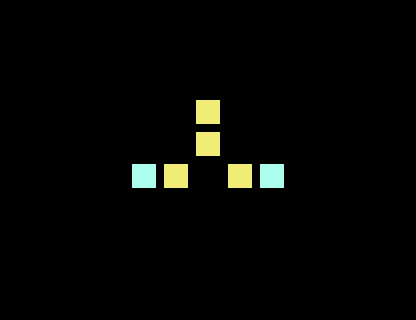
\includegraphics[width=1.3cm]{src/patterns/pixels/pixel_pattern9_2.png}%
} \\
        \midrule

        \makecell[l]{
\icode{.BYTE \$00,\$00,\$FA,\$06,\$03,\$FD}\\
\icode{.BYTE \$00,\$FC,\$FF,\$FF,\$05,\$05}
} & \makecell[l]{
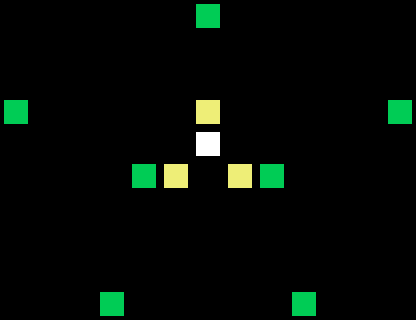
\includegraphics[width=1.3cm]{src/patterns/pixels/pixel_pattern9_3.png}%
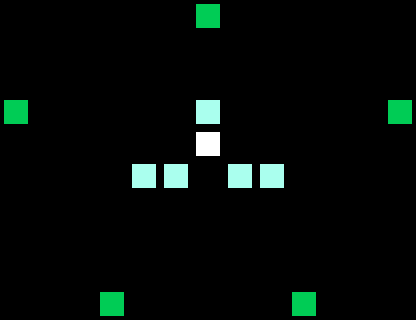
\includegraphics[width=1.3cm]{src/patterns/pixels/pixel_pattern9_4.png}%
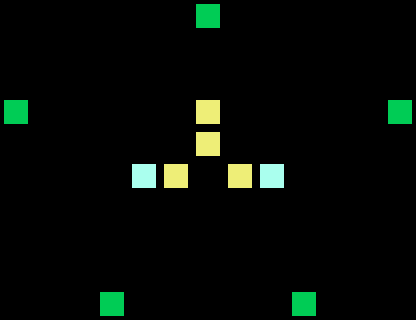
\includegraphics[width=1.3cm]{src/patterns/pixels/pixel_pattern9_5.png}%
} \\
        \midrule

        \makecell[l]{
\icode{.BYTE \$00,\$FD,\$03,\$FB,\$05}\\
\icode{.BYTE \$00,\$FD,\$FD,\$02,\$02}
} & \makecell[l]{
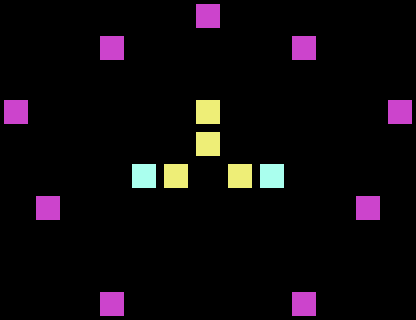
\includegraphics[width=1.3cm]{src/patterns/pixels/pixel_pattern9_6.png}%
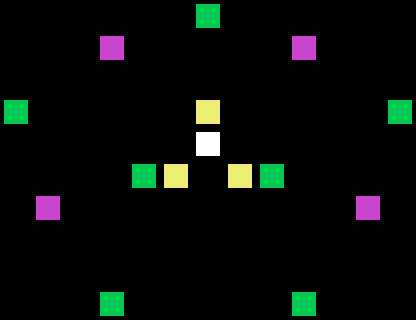
\includegraphics[width=1.3cm]{src/patterns/pixels/pixel_pattern9_7.png}%
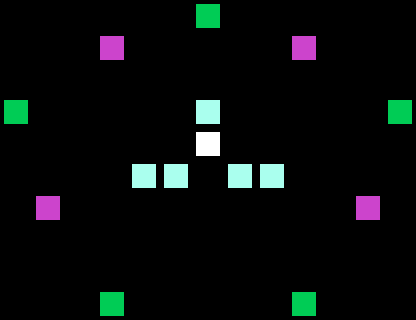
\includegraphics[width=1.3cm]{src/patterns/pixels/pixel_pattern9_8.png}%
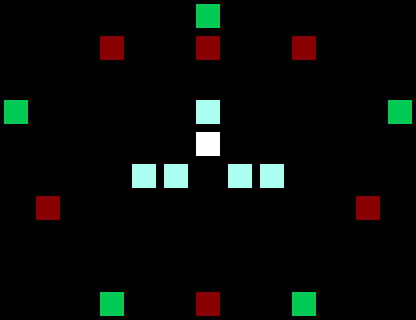
\includegraphics[width=1.3cm]{src/patterns/pixels/pixel_pattern9_9.png}%
} \\
        \midrule

        \makecell[l]{
\icode{.BYTE \$00,\$00,\$00}\\
\icode{.BYTE \$00,\$05,\$FD}
} & \makecell[l]{
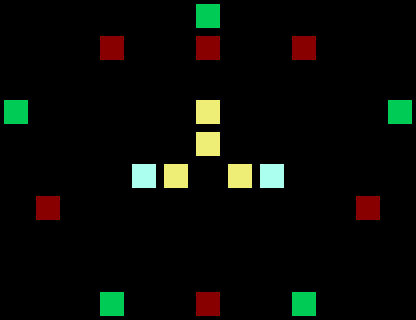
\includegraphics[width=1.3cm]{src/patterns/pixels/pixel_pattern9_10.png}%
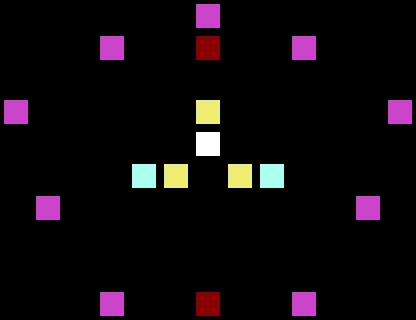
\includegraphics[width=1.3cm]{src/patterns/pixels/pixel_pattern9_11.png}%
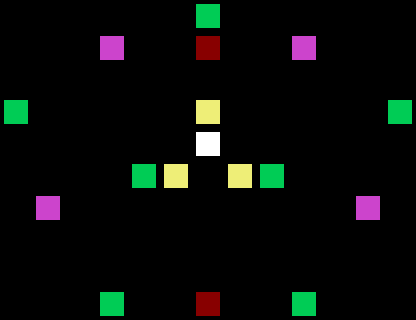
\includegraphics[width=1.3cm]{src/patterns/pixels/pixel_pattern9_12.png}%
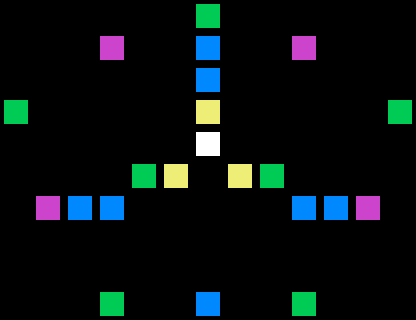
\includegraphics[width=1.3cm]{src/patterns/pixels/pixel_pattern9_13.png}%
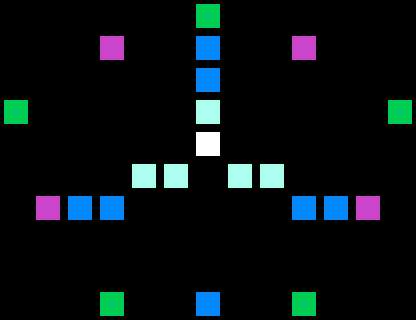
\includegraphics[width=1.3cm]{src/patterns/pixels/pixel_pattern9_14.png}%
} \\
        \midrule

        \makecell[l]{
\icode{.BYTE \$00,\$00,\$FC,\$04,\$03,\$FD}\\
\icode{.BYTE \$00,\$FE,\$02,\$02,\$02,\$02}
} & \makecell[l]{
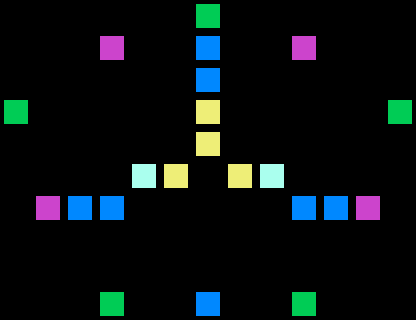
\includegraphics[width=1.3cm]{src/patterns/pixels/pixel_pattern9_15.png}%
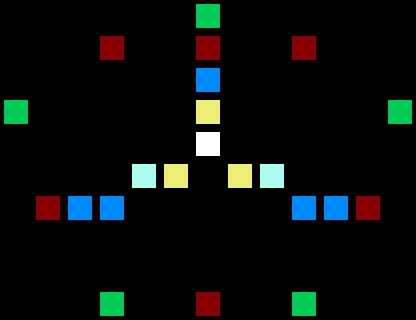
\includegraphics[width=1.3cm]{src/patterns/pixels/pixel_pattern9_16.png}%
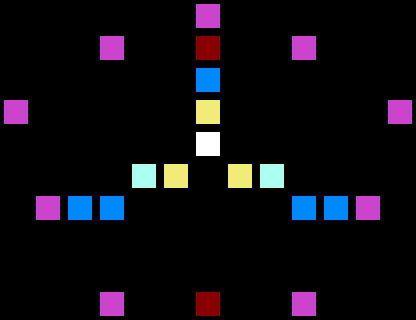
\includegraphics[width=1.3cm]{src/patterns/pixels/pixel_pattern9_17.png}%
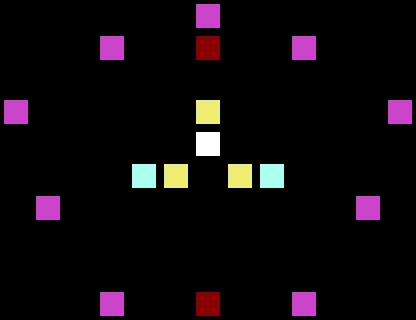
\includegraphics[width=1.3cm]{src/patterns/pixels/pixel_pattern9_18.png}%
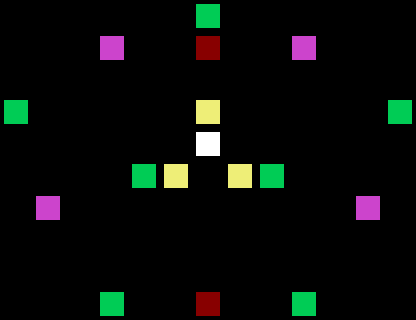
\includegraphics[width=1.3cm]{src/patterns/pixels/pixel_pattern9_19.png}%
} \\
        \midrule

        \makecell[l]{
\icode{.BYTE \$00}\\
\icode{.BYTE \$00}
} & \makecell[l]{
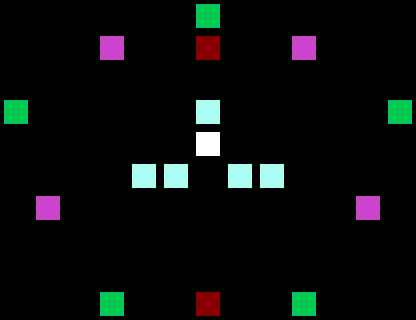
\includegraphics[width=1.3cm]{src/patterns/pixels/pixel_pattern9_20.png}%
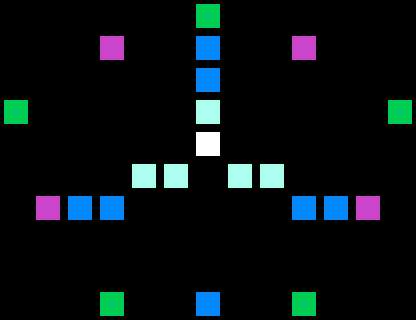
\includegraphics[width=1.3cm]{src/patterns/pixels/pixel_pattern9_21.png}%
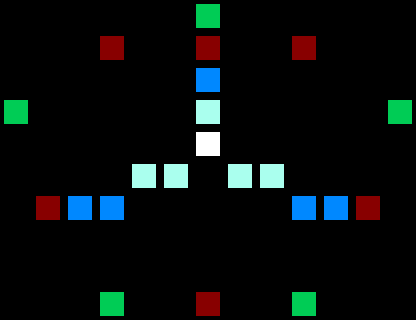
\includegraphics[width=1.3cm]{src/patterns/pixels/pixel_pattern9_22.png}%
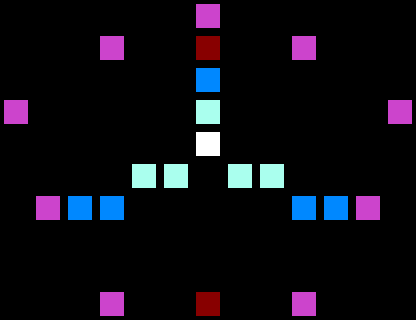
\includegraphics[width=1.3cm]{src/patterns/pixels/pixel_pattern9_23.png}%
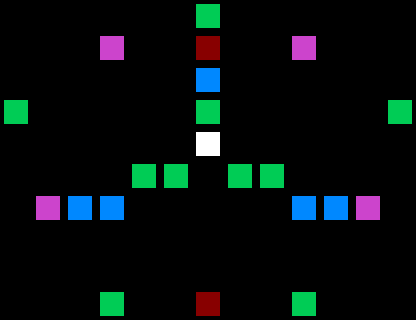
\includegraphics[width=1.3cm]{src/patterns/pixels/pixel_pattern9_24.png}%
} \\
        \midrule

      \end{tabular}
    \end{adjustbox}
  }\caption{The purpose of each of the oscillator values.}
\end{figure}
